\documentclass[12pt]{article}
\usepackage[margin=1in]{geometry} 
\usepackage{amsmath,amsthm,amssymb,amsfonts}
\usepackage{setspace}
\usepackage{mathtools}
\usepackage{graphicx}
\usepackage{float}
\singlespacing
 
\newcommand{\N}{\mathbb{N}}
\newcommand{\Z}{\mathbb{Z}}
 
\newenvironment{problem}[2][Problem]{\begin{trivlist}
\item[\hskip \labelsep {\bfseries #1}\hskip \labelsep {\bfseries #2.}]}{\end{trivlist}}
%If you want to title your bold things something different just make another thing exactly like this but replace "problem" with the name of the thing you want, like theorem or lemma or whatever
 
\begin{document}
 
\title{Homework 2 LogReg (use 3 late days, 2 left)}
\date{}
\author{Fan You}
\maketitle

\textbf{1.} How did the learning rate effect the convergence?\\

The convergence is evaluated by examining the log-likelihood function. The corresponding values for different eta values are shown below.
	\begin{figure}[H]
		\centering
		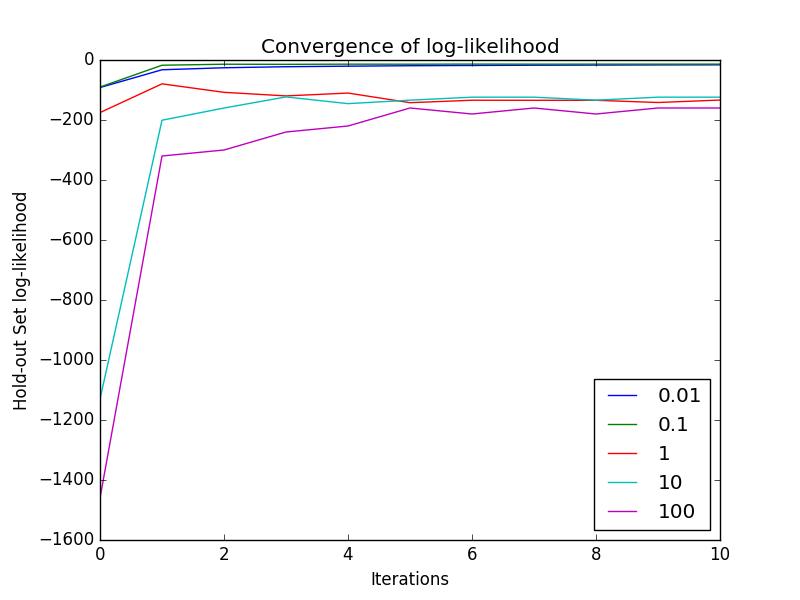
\includegraphics[scale = 0.35]{q1.png}
	\end{figure}

\textbf{2.} What was the stopping criteria and how many passes did it require?\\

The stopping criteria was set to be whenever the log-likelihood of the hold-out set stops increasing. \\

\textbf{3.} What words are the best predictors of each class?\\

The $5$ best predictors of the auto class are \texttt{car, cars, pocket, keys, warning}, since they have the lowest weights.\\

The $5$ best predictors of the motor class are \texttt{dod, bike, exhaust, bikes, ride} because they have the highest weights.\\

\textbf{4.} What words are the poorest predictors of classes?\\
The $5$ poorest predictors are \texttt{highest, heavily, horribly, gyroscoptic, medium} since they have the smallest weight in terms of absolute value.\\

\textbf{Extra Credit.} Use a schedule to update the learning rate\\

The schedule is implemented of the form $\eta_k=\frac{\eta_0}{1+\alpha k/n}$. The effect is shown below.
	\begin{figure}[H]
	\centering
	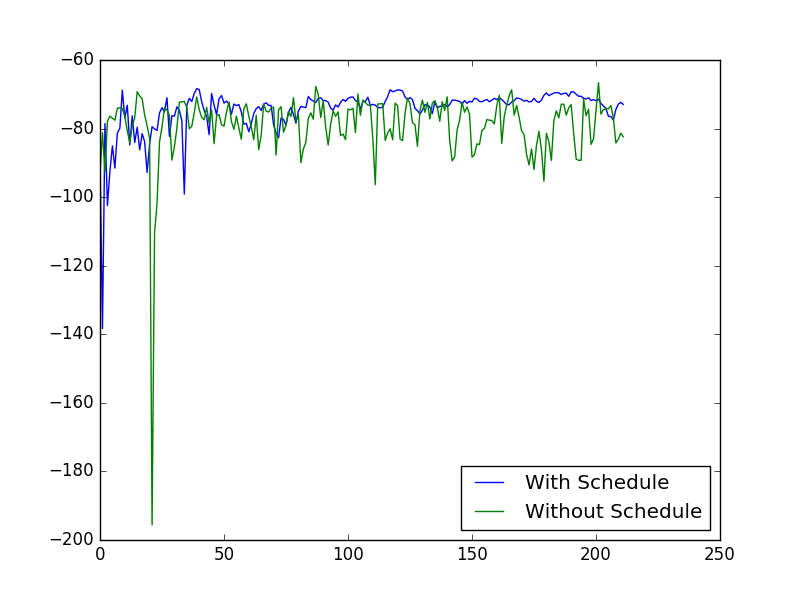
\includegraphics[scale = 0.35]{ec.png}
\end{figure}

\end{document}

















































